\chapter{The Heteronuclear Bond}

\section{Introduction}

So far, we have considered molecules formed from idential atoms, that
is, homonuclear molecules.  Now we will consider the case where the two
atoms are different, that is, heteronuclear molecules.   In this 
chapter we will examine the case of a one-electron system, then the 
two-electron case with a detailed analysis of LiH, and finally, 
the bonding of various alkali atoms and halogen atoms.

\section{The One-Electron Bond}
\subsection{Analysis of the Bond}

In Chapter 2 we considered the bonding in H$^+_2$.  In this case, the states
at $R = \infty$, $\chi_l$ and $\chi_r$, are equivalent and the linear 
combination atomic orbital, LCAO, approximation, the wavefunctions can be 
taken as $\phi_g = \chi_l + \chi_r$ and $\phi_u = \chi_l - 
\chi_r$ for all $R$.  We found, also in Chapter 2, that the
energies are of the form
\begin{equation}
\epsilon_g = \epsilon^{cl} + {\tau \over 1 + S}
\end{equation}
and
\begin{equation}
\epsilon_u = \epsilon^{cl} - {\tau \over 1 - S}
\end{equation}
where
\begin{equation}
\tau = h_{lr} - S \epsilon^{cl}
\end{equation}
\begin{equation}
h_{lr} = \langle \chi_l | h | \chi_r \rangle
\end{equation}
\begin{equation}
\epsilon^{cl} = {1 \over 2} \langle \chi_l | h | \chi_r \rangle + {1 
\over 2} \langle \chi_r | h | \chi_l \rangle
\end{equation}
\begin{equation}
h = - {1 \over 2} \nabla^2 - {Z_l \over r_a} - {Z_r \over r_b}.
\end{equation}
The $\epsilon^{cl}$ term is repulsive but small, whereas $\tau$ is large 
and negative, leading to an attractive interaction for $\phi_g$ and a 
repulsive interaction for $\phi_u$.

For a heteronuclear molecule, the exact wavefunctions at $R = \infty$ are
localized on one atom, or the other
\begin{equation}
\phi_1 = \chi_l
\label{chap17-eqno1a}
\end{equation}
or
\begin{equation}
\phi_2 = \chi_r
\label{chap17-eqno1b}
\end{equation}
since the states are no longer degenerate.  This would seem to invalidate the
entire analysis of Chapter 2, and hence, merits further consideration.

Considering just the two states of (1), the eigenstates for finite $R$ are
obtained by diagonalizing the matrix
\begin{equation}
\pmatrix{H_{11} & H_{12}\cr
H_{12} & H_{22}\cr}
\end{equation}
where $H_{ij} = \langle \phi_i | h | \phi_j \rangle .$
The eigenvalues of this matrix are
\begin{equation}
E = {(H_{11} + H_{22}) \over 2} \pm \sqrt{\left({(H_{22} - H_{11}) 
\over 2} \right)^2 + H^2_{12}}
\label{chap17-eqno2}
\end{equation}
Taking $H_{11} < H_{22}$ and $H_{12} > 0$, and defining $c$ such at
\begin{equation}
{H_{22} - H_{11} \over 2} \equiv cH_{12} ,
\end{equation}
the lower state becomes
\begin{equation}
E = H_{11} - H_{12} \left[ \sqrt{1 + c^2} - c \right]
\label{chap17-eqno3}
\end{equation}

For small $c$, we obtain $ | \Delta E | \sim H_{12}$ just as for the 
symmetric case. If $H_{12}$ is comparable to the energy splitting, $c = 
1$, we obtain
\begin{equation}
| \Delta E | = \left( \sqrt{2} - 1 \right) H_{12} = 0.4 H_{12}
\end{equation}
and for $H_{12}$ small compared with $H_{22} - H_{11}$, we obtain only a 
small bonding  effect. For example, with $c = 10$, we obtain
\begin{equation}
| \Delta E | = \left( \sqrt{101} - 10 \right) H_{12} = 0.05 H_{12} .
\end{equation}
Thus, only in the case that the energy separation of the two unperturbed
states is comparable to, or smaller than, $H_{12}$ can we expect significant 
binding.

The above analysis is oversimplified, since the atomic orbitals are not
orthogonal, $ S = \langle  \chi_l | \chi_r \rangle \not= 0$ 
and hence, the optimum wavefunction using the basis functions in 
(1), $\phi = C_l \chi_l + C_r \chi_r$
is obtained by solving for the eigenfunctions of
\begin{equation}
\pmatrix{h_{ll} & h_{lr}\cr
h_{rl} & h_{rr}} 
\pmatrix{C_l\cr
C_r} =
\pmatrix{1 & S\cr
S & 1\cr}
\pmatrix{C_l\cr
C_r} \epsilon
\label{chap17-eqno4}
\end{equation}
The resulting eigenvalues are not of the form (7), and we must re-examine
the previous analysis.

The simplest modification is to choose new orbitals $\chi_a$ and 
$\chi_b$ that are localized but orthonormal. This can be done by
\begin{equation}
\chi_a = {( \chi_l - \lambda \chi_r ) \over D}
\label{chap17-eqno5a}
\end{equation}
and
\begin{equation}
\chi_b = {( \chi_r - \lambda \chi_l ) \over D}
\label{chap17-eqno5b}
\end{equation}
where
\begin{equation}
\lambda = {(1 - \sqrt{1-S^2}) \over S} = {1 \over 2} S + O(S^3)
\label{chap17-eqno6a}
\end{equation}
and
\begin{equation}
D = \sqrt{(1 + \lambda^2) - 2 \lambda S} = \sqrt{1 - {3 \over 4} S^2} 
O(S^4) .
\label{chap17-eqno6b}
\end{equation}
In terms of the new orthogonal orbitals, the matrix equation (4) just leads
to the usual form
\begin{equation}
\underline{H}^{\prime} C = \underline{C} \epsilon
\label{chap17-eqno7}
\end{equation}
with eigenvalues as in (2).  Hence, the analysis (3) of heteronuclear binding
is valid.

Using the orthogonal basis functions (5) we obtain for the off-diagonal
matrix elements of (7)
\begin{eqnarray}
H_{12} &=& \langle \chi_a | h | \chi_b \rangle\cr
&=& {\langle l | h | r \rangle - {1 \over 2} S \left[ \langle l | h | 
l \rangle + \langle r | h | r \rangle \right] + {1 \over 4} S^2 
\langle r | h | l \rangle \over 1 - {3 \over 4} S^2} + O(S^3)\cr
&=& {\langle l | h | r \rangle - {1 \over 2} S \left[ \langle l | h | 
l \rangle + \langle r | h | r \rangle \right] \over 
(1-S^2)+O(S^3)}
\end{eqnarray}
where
\begin{equation}
\tau = \langle l | h | r \rangle = {2 \over 2} S \left[ \langle l | h 
| l \rangle  + \langle r | h | r \rangle \right]
\end{equation}
has the same form as in the homonuclear case. This should be compared
with
\begin{equation}
\Delta \epsilon_g = {\tau \over 1 +S}
\end{equation}
for the bonding, $\sigma_g$, state in H$^+_2$, and
\begin{equation}
\Delta \epsilon_u = {- \tau \over 1 - S}
\end{equation}
for the antibonding, $\sigma_u$, state.  Indeed, for H$^+_2$ the 
separation between the bonding and antibonding states is
\begin{equation}
\Delta E = {2 \tau \over 1 - S^2} ,
\end{equation}
which is twice the off-diagonal element (6) for the heteronuclear case.

In the limit that $(H_{11} - H_{22}) \rightarrow 0$ the bond energy of the 
bound state is $-H_{12}$ and the repulsive energy of the higher state 
is $+H_{12}$.  Thus, the
origin of the bond for the heteronuclear case arises from the same 
term $\tau$ responsible for the bond in the homonuclear case.

\subsection{Applications}

\subsubsection{HeH$^{++}$}

Consider, first, the case of HeH$^{++}$.  At $R = \infty$, the energy of 
$\chi_l$, on the He, is $E_l = -2.0$ while the energy of $\chi_r$, on 
the H, is $E_r = -0.5$.  Thus, the separation $H_{rr} - H_{ll} = 1.5h =
40.8$eV is large compared to the range of
values for $H_{12}$, say 4 eV, and no significant bonding is expected.

More importantly the energy of $H_{ll}$ depends on $R$ as
\begin{equation}
H_{ll} = - 2.0 + {1 \over R}
\end{equation}
since there is a net charge on each atom.  Thus, the potential curve for the
ground state of HeH$^+$ should be quite repulsive.

Since the first excited state of He, $2s$ and $2p$, $E = -0.5$, is degenerate
with the $1s$ state of H, we might expect a significant bonding effect. Thus,
$H_{12}$ is probably $\sim$4 eV for $R$ around $1a_0$.  However, the 
classical energy for the term in which the electron is on the He, behaves as
\begin{equation}
E = - 0.5 + {1 \over R} .
\end{equation}
Even at $R = 3a_0$, the value of $1/R$ is 1/3 Hartree = 9 eV, and hence, the
classical energies are quite different, i.e., large $H_{22} - H_{11}$.  Thus, 
a bond is not expected.  The second state of HeH$^+$ would correspond to 
an electron mainly on the H and would probably lead to a flat potential 
curve, whereas the ground state and the third and fourth state, at 
larger $R$, would be quite repulsive.

\subsubsection{LiH$^+$}

As another example, consider LiH$^+$.  Although there are three electrons
here, two are Li core orbitals and are essentally unchanged for the range of
internuclear separations of interest here.  For $R \rightarrow 0$, 
LiH$^+ \rightarrow$ H$^+$, and hence, large changes must occur also 
in the core orbitals.  Thus, effectively LiH$^+$ is a one-electron system.

The lower states at $R = \infty$, are:
\begin{eqnarray}
H1s = \epsilon &=& -0.5\cr
Li2s = \epsilon &=& -0.196\cr
Li2p = \epsilon &=& -0.128\cr
H2s, 2p \epsilon &=& -0.125
\end{eqnarray}
and,
\begin{equation}
Li3s = \epsilon = -0.076.
\end{equation}
In this case, there are no net $1/R$ terms for large $R$.  However, the 
separation of the first two states is large compared with the expected 
size of $H_{12}$, and
hence, no strong chemical bond is expected.  Indeed, the resulting bond
energy is only 0.1 eV, with an optimum $R$ of $\sim4.5 a_0$.

\subsection{An Alternative Analysis}

We will now examine the heteronuclear bond from a slightly different
point of view, using non-orthogonal basis functions.

Assuming that $\chi_l$ has a lower energy than $\chi_r$, we write the optimum
orbital at finite $R$ as $\phi = C_l \chi_l + C_r \chi_r$.  Since 
$\phi$ is normalized, we have
\begin{equation}
1 = C_l + C^2_r + 2C_l C_r S
\label{chap17-eqno8}
\end{equation}
where $S = \langle \chi_l | \chi_r \rangle$. The energy of $\phi$ is
\begin{equation}
E = C^2_l H_{ll} + C^2_rH_{rr} + 2 C_lC_rH_{lr},
\label{chap17-eqno9}
\end{equation}
where $H_{ll} = \langle \chi_l | {\cal H} | \chi_l \rangle$,
etc.  Using (8), we can write (9) as
\begin{equation}
E = H_{ll} + C^2_r \left( H_{rr} - H_{ll} \right) + 2 C_l C_r \left( 
H_{lr} - SH_{ll} \right).
\end{equation}
The quantity $(H_{rr} - H_{ll})$ is positive, whereas the quantity 
$\tau = H_{lr} - SH_{ll}$ is expected to be negative.  Thus, the strength 
of the bond is determined by the size of $\tau$ just as for the 
homonuclear case.

For the case of a strong bond, we expect
\begin{equation}
C_l = C_r = {1 \over \sqrt{2(1+S)}} ,
\end{equation}
and, hence
\begin{equation}
\Delta E = {1 \over 2(1+S)} \left[ 2 \tau + \left( H_{rr} - H_{ll} 
\right) \right] .
\end{equation}
Note that $\tau$ and $\Delta E$ are negative so that large $H_{rr} - 
H_{ll}$ leads to a decrease in the bond energy.

About the only case for which this analysis is interesting, is that of
alkali metals Li$^+$, LiNa$^+$, etc., where the ionization potentials are similar
enough to get moderately strong bond, $\sim$1 eV.  In cases with additional net
charges, the overall net Coulomb interactions dominate the bonding effects
as illustrated above for HeH$^{++}$.

\section{The Two-Electron Bond}

We will now consider a heteronuclear molecule with one valence 
electrons on each center, using LiH as a prototype.

\subsection{The Wavefunctions of LiH}

First we will examine the energies from various calculations on LiH.
In the next section, we will then analyze these wavefunctions.

We will consider wavefunctions of the form
\begin{equation}
{\cal A} \left[ \phi_1 \phi_1 \left( \phi_2 \phi_3 + \phi_3 \phi_2 
\right) \alpha \beta \alpha \beta \right] ,
\end{equation}
where for $R = \infty$, $\phi_1$ describes the $1s$ core orbitals of the 
Li, $\phi_2$ describes the $2s$ valence orbital of the Li and $\phi_3$ 
describes the $1s$ valence orbital of the hydrogen.  For finite $R$ we 
will consider four types of wavefunctions, all
making use of a minimal basis of atomic orbitals.

For valence bond, VB:
\begin{eqnarray}
\phi_1 &=& \chi^{Li}_{1s}\cr
\phi_2 &=& \chi^{Li}_{2s}\cr
\phi_3 &=& \chi^{H}_{1s}
\end{eqnarray}

For hybridized valence bond, VB-H:
\begin{eqnarray}
\phi_1 &=& \chi^{Li}_{1s}\cr
\phi_3 &=& \chi^H_{1s}\cr
\phi_3 &=& C_s \chi^{Li}_{2s} + C_p \chi^{Li}_{2p_z}
\end{eqnarray}

For generalized valence bond, but with a fixed core orbitals, GVB-FC:
\begin{equation}
\phi_1 = \chi^{Li}_{1s}
\end{equation}
$\phi_2$ and $\phi_3$ allowed to use any combination of 
$\chi^H_{1s}$, $\chi^{Li}_{2s}$, and $\chi^{Li}_{2p_z}$. 

For generalized valence bond, GVB, all orbitals allowed to use any
combination of the Li$1s$, $2s$, $2P_z$, and $H1s$ orbitals.

In all of these calculations, only the four atomic orbitals are used.
That is, a minimal basis set of atomic orbitals, and hence, the calculation 
for generalized valence bond does not correspond to a full generalized valence
bond calculation.  However, the major influences on the bonding are manifest.

The calculated energies are shown in Figure \ref{chap17-fig1}.  All
wavefunctions use a minimal basis set of atomic orbitals. The valence
bond wavefunction above accounts for 45 percent of the generalized
valence bond energy. Allowing the Li orbital to hybridize, VB-H, leads
to a drastic improvement, accounting for about 80 percent of the
generalized valence bond energy. Freezing the Li$1s$ orbital in the
generalized valence bond calculations, has only a minor effect so that
the generalized valence bond-fixed core and generalized valence bond
curves superimpose in Figure \ref{chap17-fig1}.

Contour plots of the orbitals corresponding to these four cases, are
shown in Figure \ref{chap17-fig2} for the case of $R = 3.2a_0$.  Line
plots of these cases, are shown as a function of $R$ in Figure
\ref{chap17-fig3}.

The calculated bond lengths and bond energies, are given in Table
\ref{chap17-tab2a}--\ref{chap17-tab2b}.  Also include here, are the
results of calculations using more extended basis sets. The potential
curves for the extended basis case are shown in Figure \ref{chap17-fig4}.

\begin{figure}
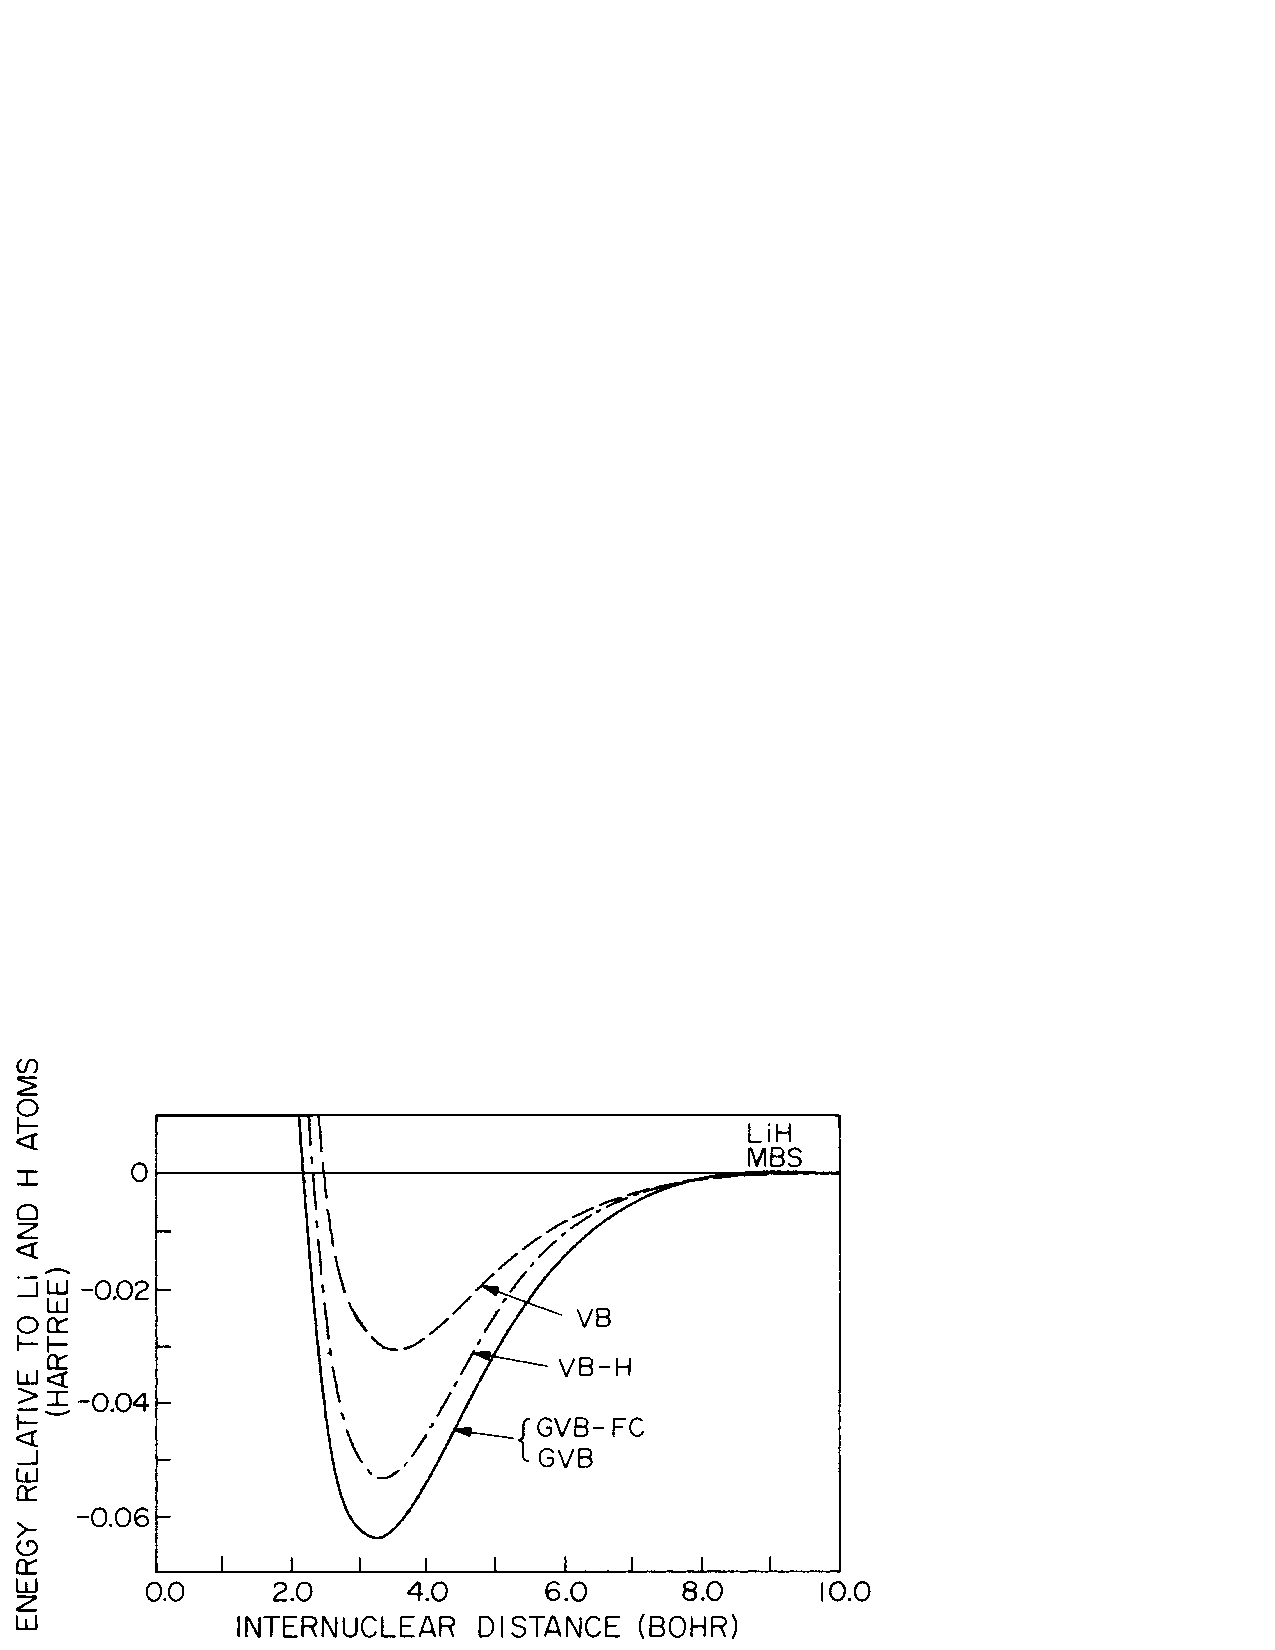
\includegraphics[scale=0.75]{fg17-1}
\caption{Energy curves for LiH.}
\label{chap17-fig1}
\end{figure}

\begin{figure}
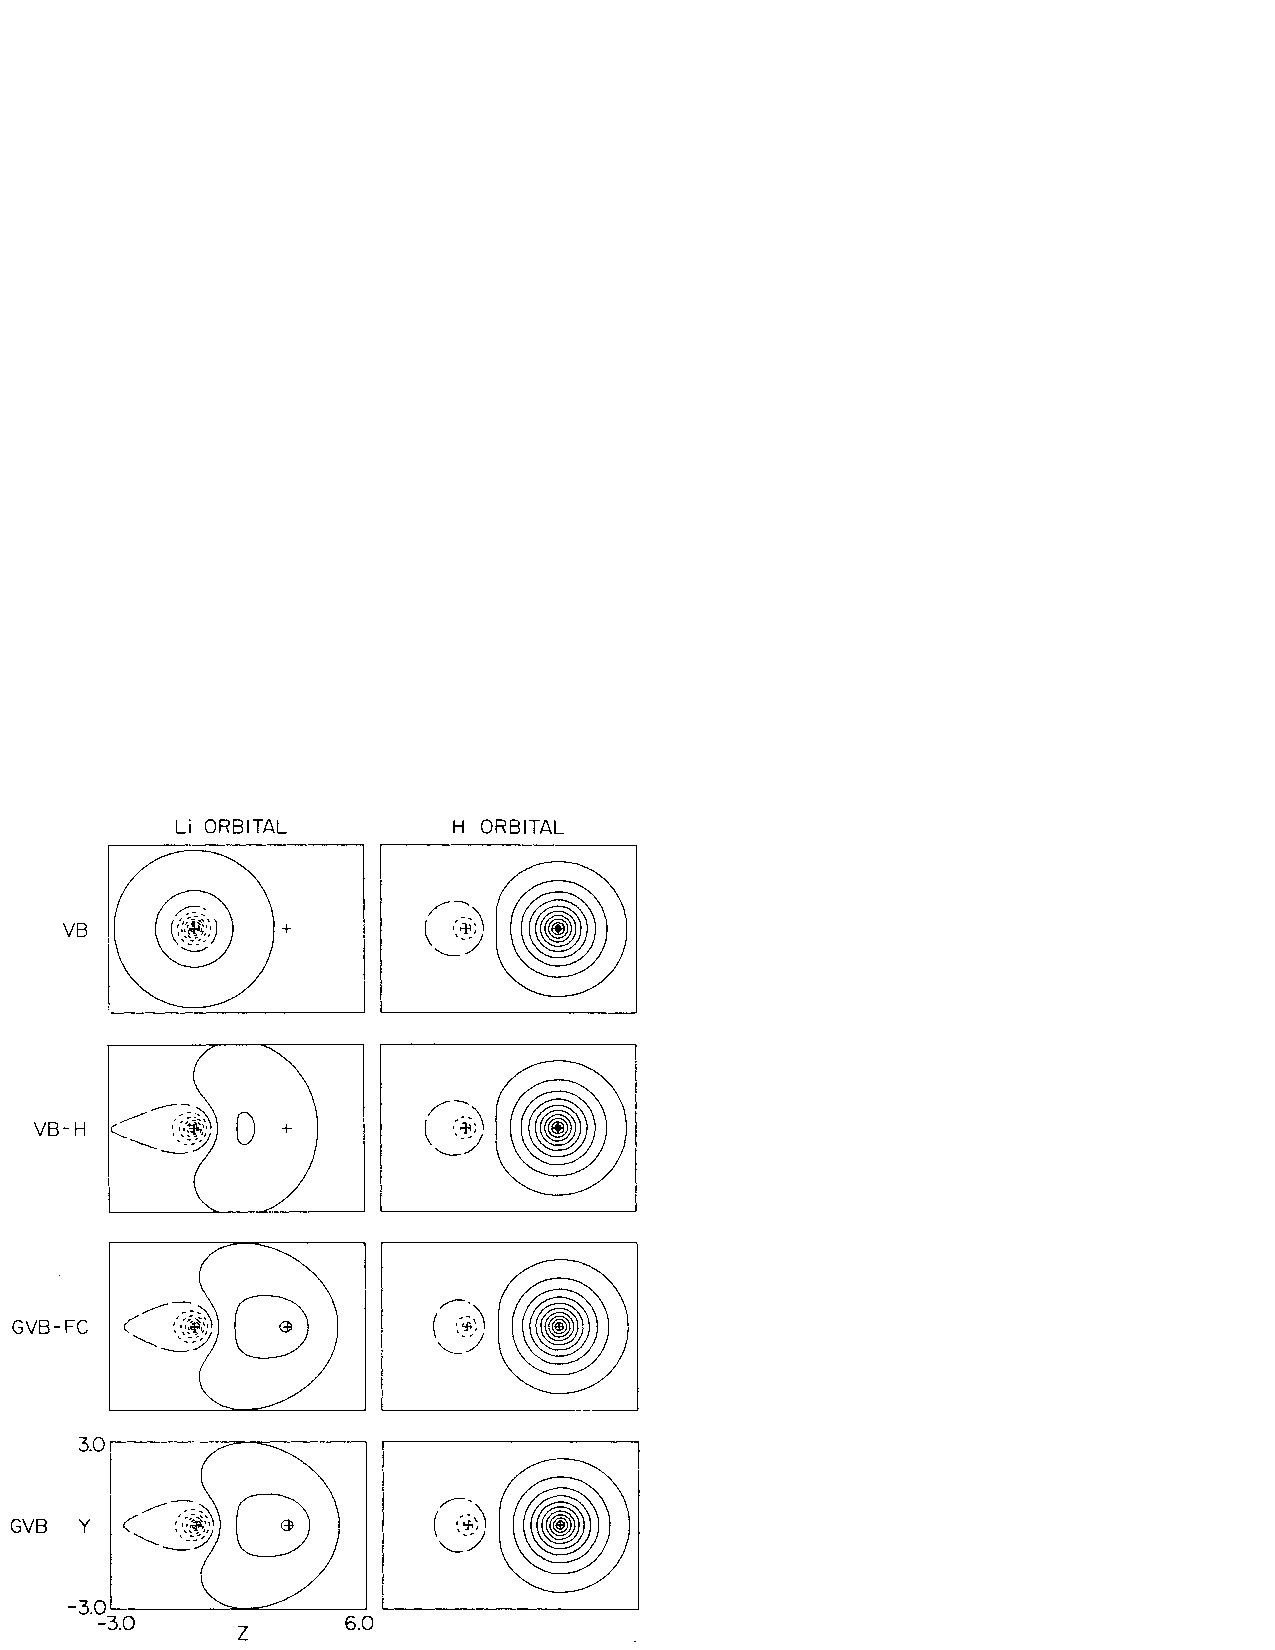
\includegraphics[scale=0.75]{fg17-2}
\caption{The orbitals for LiH at $R = 3.2a_0$ (minimal basis set).} 
\label{chap17-fig2}
\end{figure}

\begin{figure}
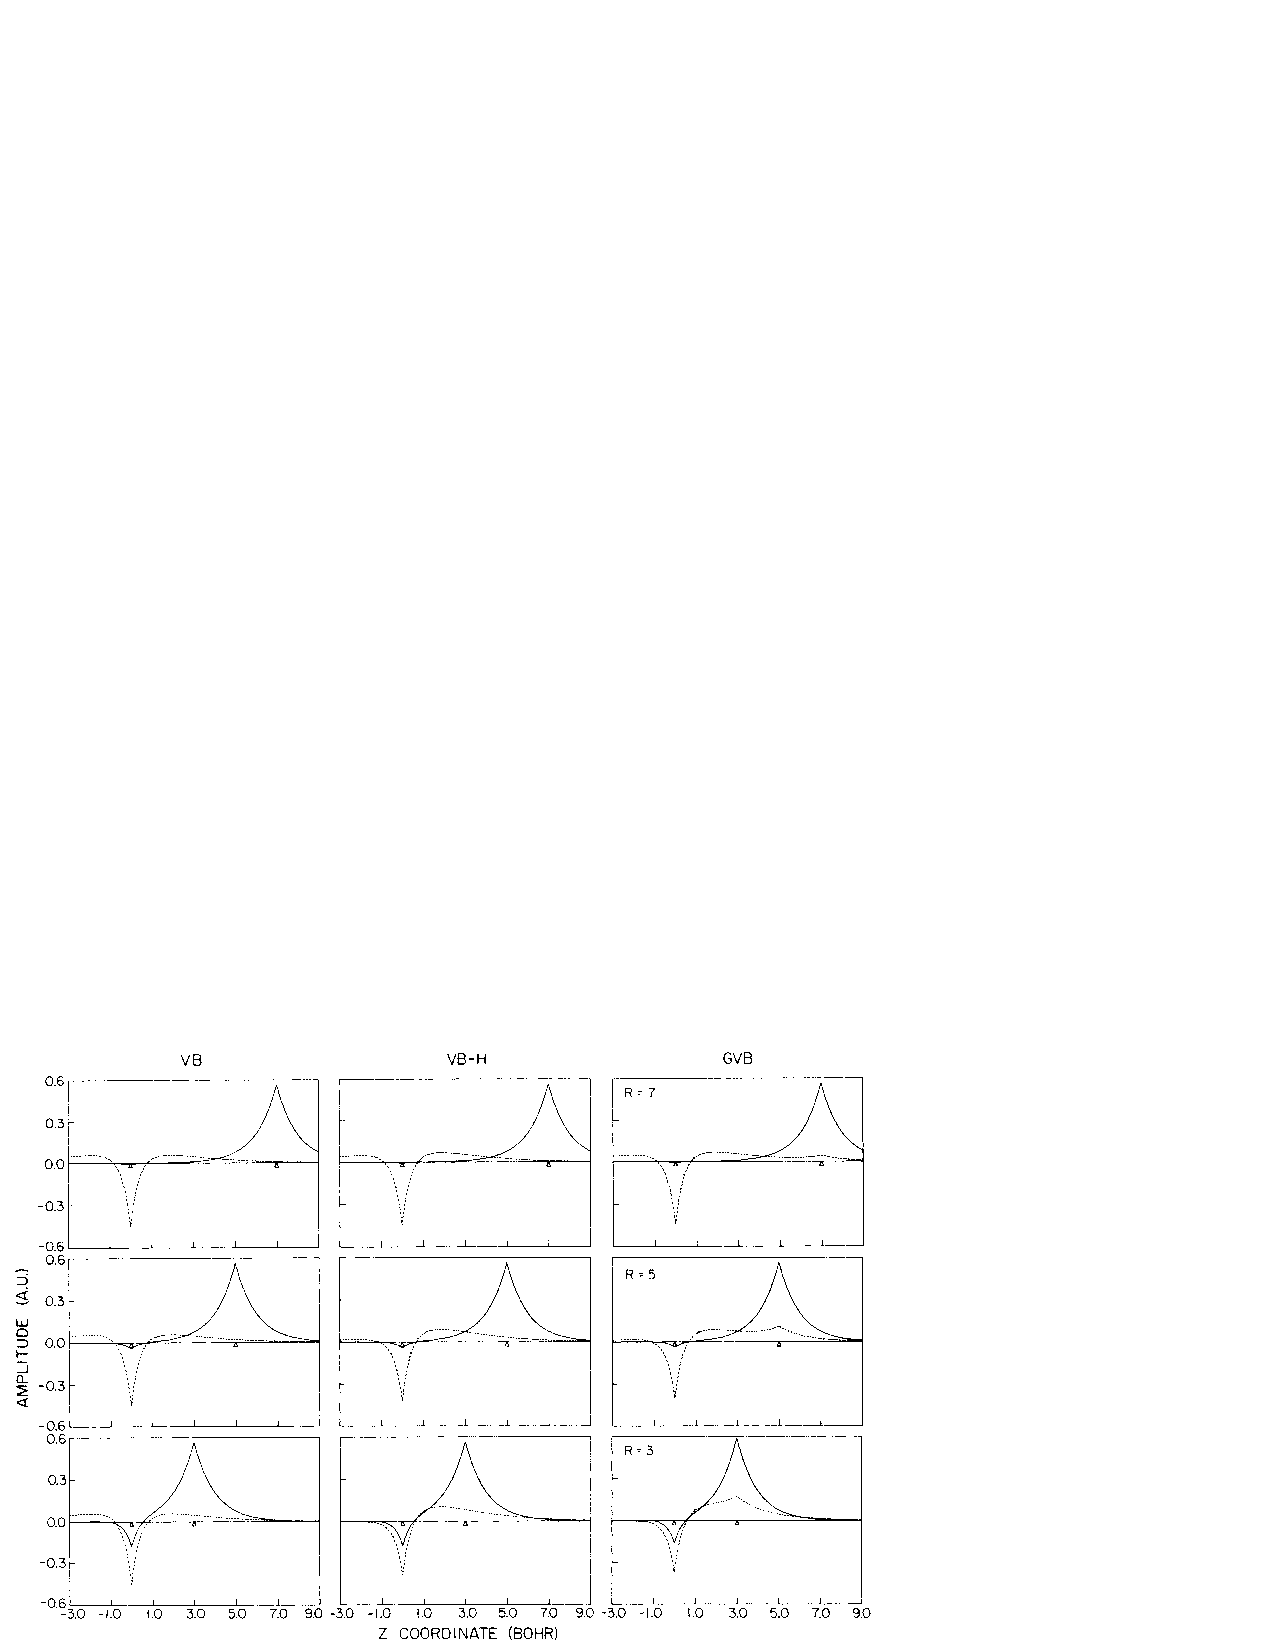
\includegraphics[scale=0.75]{fg17-3}
\caption{VB and GVB orbitals of LiH as a function of $R$ (minimal
basis set).}
\label{chap17-fig3}
\end{figure}

\begin{figure}
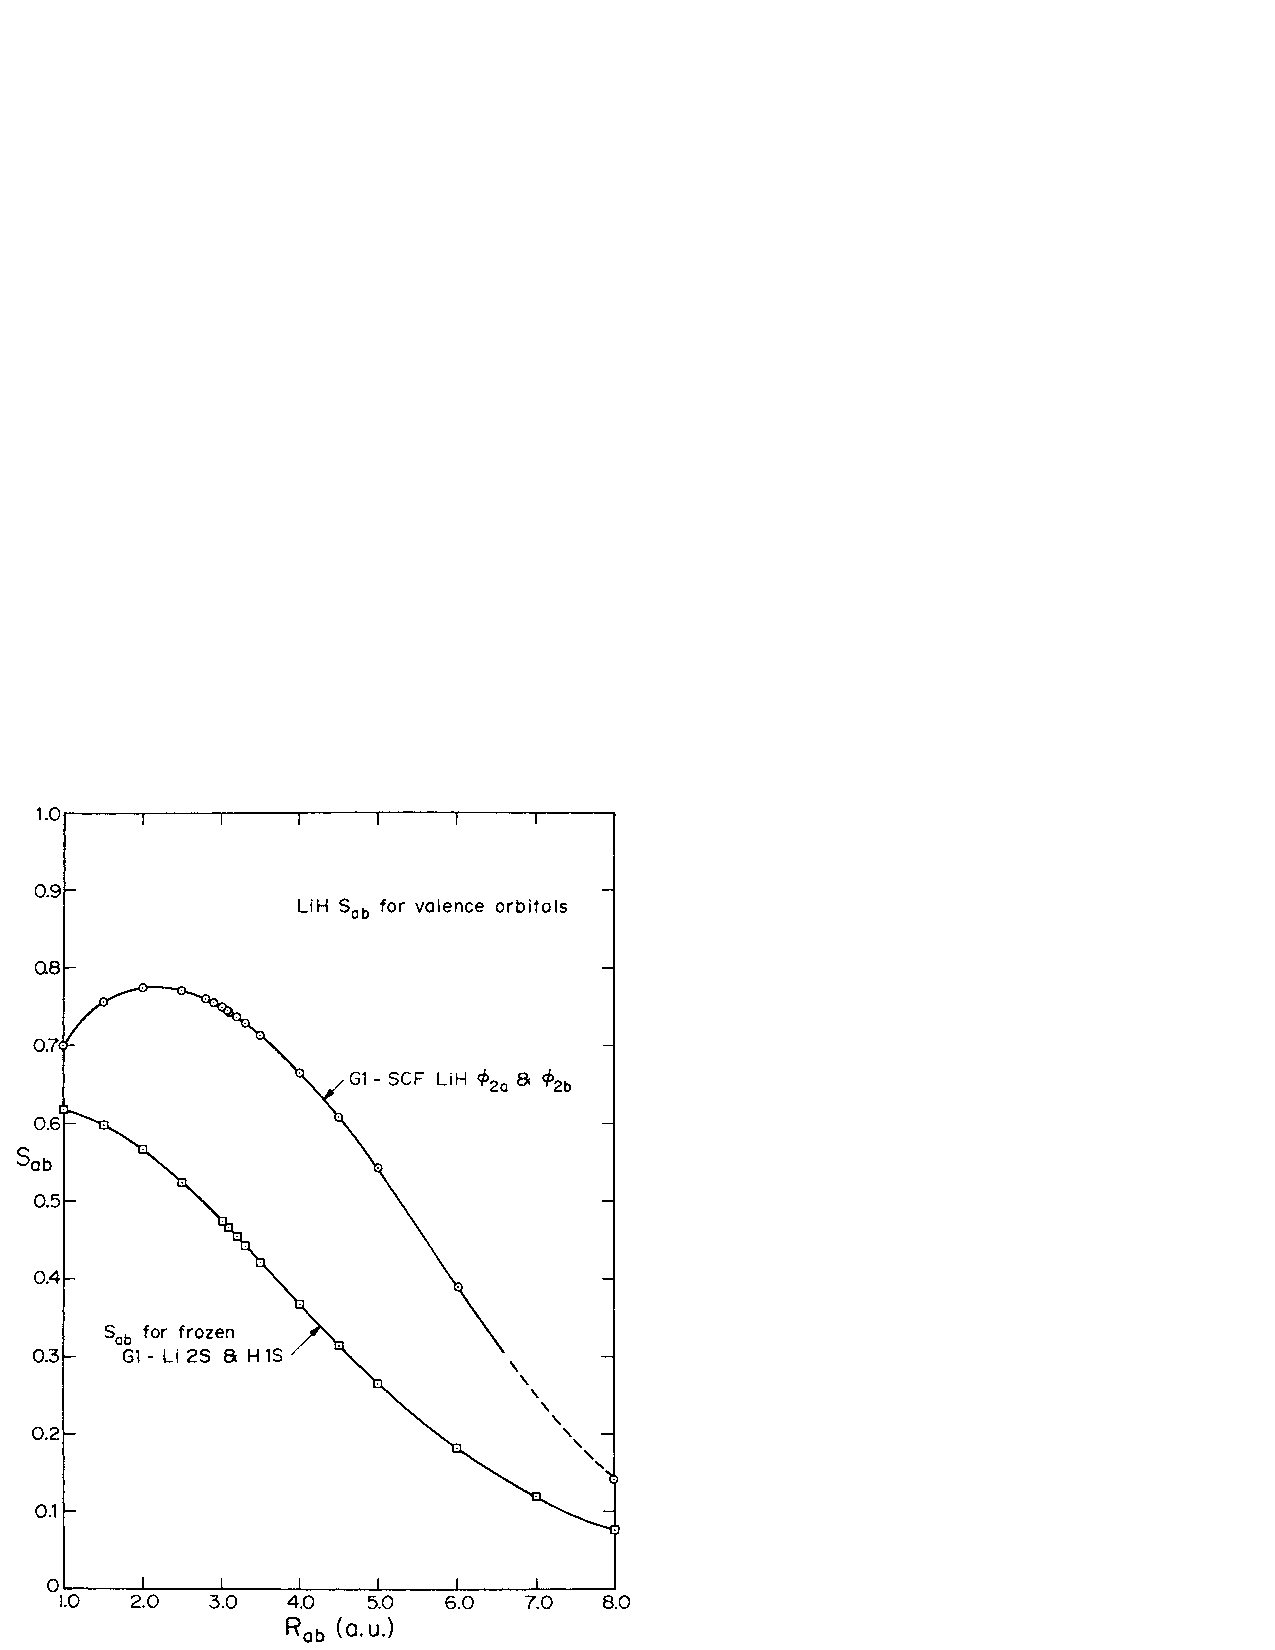
\includegraphics[scale=0.75]{fg17-4}
\caption{Comparison of the overlap of valence orbitals for 
the VB and GVB wavefunctions.}
\label{chap17-fig4}
\end{figure}

\begin{table}
\caption{Expansion coefficient for the wavefunctions of 
LiH, all for minimal basis function sets. Slater type orbitals,
exponents in parentheses.}
\label{chap17-tab1}
\begin{tabular}{cccccc}\\ \hline
& & Li$1s$ & Li$2s$ & Li$2p_z$ & $H1s$\cr
& & (2.6906) & (0.6396) & (0.6396) & (1.0)\cr

VB & $\phi_{1s}$ & 0.99717 & 0.01659 & 0.0 & 0.0\cr
& $\phi_{2s}$ & $-$0.18122 & 1.01336 & 0.0 & 0.0\cr
& $\phi_H$ & $-$0.04353 & $-$0.00072 & 0.0 & 1.00095\cr
VB-H & $\phi_2$ & $-$0.16084 & 0.89941 & 0.46070\cr
GVB-FC & $\phi_2$ & $-$0.15162 & 0.80690 & 0.41338 & 0.16788\cr
& $\phi_3$ & $-$0.04638 & $-$0.02291 & $-$0.02638 & 1.02163\cr
GVB & $\phi_{1s}$ & 0.99698 & 0.01755 & $-$0.00124 & 0.00038\cr
& $\phi_2$ & $-$0.15205 & 0.80678 & 0.41354 & 0.16790\cr
& $\phi_3$ & $-$0.04059 & $-$0.02291 & $-$0.02636 & 1.02162\cr
\hline
\end{tabular}
\end{table}

\begin{table}
\caption{Calculated geometric parameters for LiH, minimal basis set.}
\label{chap17-tab2a}
\begin{tabular}{ccccc}\\ \hline
& VB & VB-H & GVB-FC & GVB\cr

$E(R_e)$ & $-$7.94946 & $-$7.97222 & $-$7.98259 & $-$7.98263\cr
$D_e(h)$ & 0.03098 & 0.05374 & 0.06411 & 0.06415\cr
$R_e(a_0)$ & 3.510 & 3.323 & 3.241  & 3.239\cr	

\hline
\end{tabular}
\end{table}

\begin{table}
\caption{Calculated geometric parameters for LiH, extended basis.}
\label{chap17-tab2b}
\begin{tabular}{ccccc}\\ \hline
& HF$^a$ & GVB$^b$ & CI$^c$ & Experiment\cr

$E(R_e)$ & $-$7.98732 & $-$8.01754 & $-$8.0606 & $-$8.0705\cr
$D_e(h)$ & 0.0545 & 0.0701 & - & 0.0926\cr
$R_e(a_0)$ & 3.034 & 3.092 & - & 3.015\cr
\hline
\end{tabular}\\
$^a$ See reference 2.
$^b$ See reference 3.
$^c$ See reference 4.
\end{table}

\subsection{Analysis of Hybridization}

In the hybridized valence bond wavefunction, only the $\phi_2$ orbital, 
denoted as $\psi_{sp}$, departs from the atomic form,
\begin{equation}
\phi_{sp} = 0.88756 \chi_{2s} + 0.46070 \chi_{2p_z}
\end{equation}
where $\chi_{2s}$ refers to the Li$2s$ atomic orbital, not just the 
$2s$ Slater orbital.  That is, the hybridized orbital has 21.2 percent 
$p$ character.  This small
amount of hybridization has a large effect upon the overlap of 
$\phi_{sp}$ with the $\phi_H$ orbital, and in turn, upon the bond energy.

The atomic overlaps are $S_{2s,H} = 0.36974$ and $S_{2p_z},H = 
0.49035$, and hence, the hybridized orbital leads to $S_{sp,H} = 
0.55407$, a 49.9 percent increase despite the fact that only 21.2 
percent $p$ character is introduced.

The $T^x$ between orbitals $a$ and $b$ is
\begin{equation}
T^x = - {S^2 \over 1 + S^2} \left[ t_{aa} + t_{bb} - {2t_{ab} \over 
S} \right]
\label{chap17-eqno10}
\end{equation}
As indicated in Tables \ref{chap17-tab2a}--\ref{chap17-tab2b}, the
$2p$ and $2s$ orbitals, with the same exponent, have similar kinetic
energies, and hence, so does the hybridized orbital.  In addition, we
note that $t_{ab}/S$ is nearly the same for either choice of Li
orbitals,
\begin{equation}
{t_{2p,H} \over S_{2p,H}} = 0.14627
\end{equation}
while
\begin{equation}
{t_{2s,H} \over S_{2s,H}} = 0.15568
\end{equation}
so that hybridizing the orbital leads to little change in the bracketed 
quantity of (10).  However,
\begin{equation}
{S^2 \over (1+S)} = 0.09981
\end{equation}
for the $\phi_{2s}$, orbital, and
\begin{equation}
{S^2 \over (1+S)} = 0.19754
\end{equation}
for the hybridized orbital, a factor of 1.9792 increase. Since $T^x$ dominates
bonding, we expect a large increase in the bond energy.  As shown in Table
\ref{chap17-tab3}, $\Delta E$ increases from $-$0.0284 to $-$0.0454,
an increases of 59.9 \%.

\begin{table}
\caption{Analysis of LiH wavefunctions at $R = 4a_0$.  
Here $\Delta E = E(R=4)-E(R=\infty)$ and similarly for other quantities.}
\label{chap17-tab3}
\begin{tabular}{cccc}\\ \hline
 & VB & VB-H & GVB-FC\cr

$S$ & 0.36974 & 0.55407 & 0.64675\cr
$\Delta E^{Cl}$ & $-$0.00317 & $-$0.00195 & $-$0.01641\cr
$\Delta E^x$ & $-$0.02525 & $-$0.04346 & $-$0.03742\cr
$\Delta E$ & $-$0.02840 & $-$0.04542 & $-$0.05382\cr
$\Delta T^{Cl}$ & 0.00844 & 0.00374 & 0.01514\cr
$\Delta V^{Cl}$ & $-$0.01161 & $-$0.00569 & $-$0.03155\cr
$\Delta T^x$ & $-$0.05098 & $-$0.10023 & $-$0.07526\cr
$\Delta V^x$ & 0.02573 & 0.05677 & 0.03784\cr
$\Delta V^{enx}$ & 0.00389 & 0.02922 & 0.00535\cr
$\Delta V^{eex}$ & 0.02184 & 0.02755 & 0.03249\cr
\hline
\end{tabular}
\end{table}

The lesson here is that relatively small amounts of hybridization in an
orbital, can lead to a large increase in the overlap with orbitals on 
adjacent atoms.  For this to be energetically favorable, it must be that the 
excitation energy to this hybridizing orbital, $px$ for Li, is relatively 
small.  Basically, we will find that the most effective hybridizing orbitals 
are those of the same n quantum number, and one additional nodal plane 
perpendicular to the $Z$ axis, assuming a bond along the $Z$ axis. Thus, 2 
uses $2p$, $3s$ uses $3p$, and $3p$ uses $3d$, etc.

\subsection{Analysis of Ionic Character}

Allowing the Li valence orbital to delocalize onto the hydrogen, led to
an additional 18 percent in the bond energy and larger changes in the 
classical and exchange energies.  These calculations also allowed the 
hydrogen orbital to delocalize but this effect was less important.

First, we will make a generally analysis using LiH as the prototype.
We assume that the $\chi_H$ orbital remains fixed and allow the Li orbital to
delocalize $\phi_{sp,H} = C_1 \phi_{sp} + C_2 \phi_h$ 
where $C_1 = 0.89714$, and $C_2 = 0.16788$ for LiH at $4a_0$.

Second, we will consider only the classical terms, that is the energy terms
corresponding to $\phi_1 \phi_1 \phi_{sp,H} \phi_H$. The energy of this 
wavefunction is
\begin{equation}
E^{Cl} = 2 \langle 1 | h | 1 \rangle + \langle spH | h | spH 
\rangle + \langle H | h | H \rangle + J_{11} + 2J_{1,spH} + 2J_{1,H} + 
J_{spH,H} + {3 \over R}
\end{equation}
and the change in the energy due to delocalization onto the hydrogen, is
given by
\begin{equation}
\Delta E = D^2_2 \left( H_{HH} - H_{sp,sp} \right) + 2 C_1C_2 \left( 
H_{H,sp} - S_{sp,H} H_{sp,sp} \right)
\label{chap17-eqno11}
\end{equation}
where
\begin{eqnarray}
H_{sp,sp} &=& \langle \phi_{sp} | \left( h + 2J_1 + J_H \right) | 
\phi_{sp} \rangle\cr
H_{H,H} &=& \langle \phi_H | \left( h + 2J_1 + J_H \right) | 
\phi_H \rangle\cr
H_{H,sp} &=& \langle \phi_H | \left( h + 2J_1 + J_H \right) | 
\phi_{sp} \rangle
\end{eqnarray}
This is just as if we had a one-electron system in which the Li$1s$ and 
H$1s$ orbitals were replaced by the Coulomb fields $J_1$ and $J_H$.

A crude estimate of $H_{HH} - H_{sp,sp}$ can be made as follows.  This is the
change in the energy due to ionizing an electron from the $sp$ orbital, this
costs $0.79 \times 0.20h + 0.21 \times 0.13h = 0.185$, and placing it on 
the $H$.  For our minimum basis set, the energy of $H^-$ is
$2 \epsilon_H + J_{1s,1s} = 2 (-0.5) + 0.625 = -0.375$
and thus, at $R = \infty$ we expend another $0.25h$ to place the electron on the
$H$.  However, for finite $R$, the electron on the $H^-$ still sees the 
$-1/R$ net potential due to the Li core and hence, we expect
\begin{equation}
H_{HH} = H_{sp,sp} = 0.2 + 0.125 - {1 \over R} = 0.075h
\end{equation}
for $R = 4a_0$.  Actual calculation, see Table \ref{chap17-tab4},
leads to $H_{HH} - H_{sp,sp} = 0.6398h$.  That is for smaller $R$, the
increase in energy due to transferring an electron from one atom to
another is relatively small since the electron, on the second center,
still experiences about the same Coulomb attraction as when centered
upon the first atom.

\begin{table}
\caption{Quantities involved in analyzing the ionic contributions 
to $E^{Cl}$, for LiH at $R = 4a_0$.$^a$}
\label{chap17-tab4}
\begin{tabular}{ccccccc}\\ \hline
Q & $t$ & $v^{en}$ & $2J_{1s}$ & $J_H$ & $V^b$ & $+V$\cr

$Q_{sp.sp}$&0.22199&$-$1.34269&0.64438&0.29217$^c$&$-$0.40614&$-$0.18415\cr
$Q_{H,H}$&0.50844&$-$1.75367&0.49910&0.62596&$-$0.62801&$-$0.12017\cr
$Q_{sp,H}$&0.08413&$-$0.82333&0.31714&0.26018&$-$0.24602&$-$0.16189\cr
$Q_{HH}-Q_{spsp}$&0.28645&$-$0.41098&&&$-$0.22247&0.06398\cr
$\lambda^2_2(Q_{HH}-Q_{spsp})$&0.00807&$-$0.01158&&&$-$0.00627&0.00180\cr
$Q_{spH}-S_{spH}Q_{spsp}$&$-$40.03887&$-$0.07939&&&$-$0.02099&$-$0.05986\cr
$2\lambda_1 \lambda_2$&$-$0.01171&$-$0.02391&&&$-$0.00632&$-$0.01803\cr
$\Delta Q^{Cl}$ &$-$0.00364&$-$0.03550&&&$-$0.01259&$-$0.01623\cr
\hline
\end{tabular}\\
$^a$ Here $S = 0.55407$, $\lambda^2_2 = 0.02818$, and $2 
\lambda_1 \lambda_2 = 0.30124$.
$^b$ $V = v^{en} + 2J_{1s} + J_H$.
$^c$ $K_{sp,H} - 0.12263$.
\end{table}

Now that we know the repulsive term of (11) to be relatively innocuous,
we shift our attention to the attractive term $2C_1C_2(H_{H,sp} - 
S_{sp,H} H_{sp,sp})$.   We immediately recognize that
\begin{equation}
H_{H,sp} - S_{sp,H} H_{sp,sp}
\label{chap17-eqno12}
\end{equation}
as a $\tau$-like term.  From Table \ref{chap17-tab4}, we see that the
total value of (12) is $-0.05986h$, whereas the one-electron part is
$-0.11826$.

Summarizing, we find that the ionic part of the wavefunction, leads
to a large decrease in the classical part of the energy due, mainly, to 
one-electron $\tau$-type terms.  Significant ionic character is possible 
at smaller $R$, since the transferred electron remains close enough to 
the original center to experience a very significant $-1/R$ Coulomb potential.

\subsection{Qualitative Relationship}

In Chapter 2, we found that the bond energy of H$_2$, for larger $R$, is
approximately
\begin{equation}
\Delta E = - {2S^2 \over 1+SA^2}C
\end{equation}
where $C$ is roughly independent of $R$.  For a heteronuclear bond, 
$\Delta E$ is again dominated by $\tau$, and we may expect a smaller 
relationship.  For atomic orbitals, with unequal exponents, $\zeta_a$ 
and $\zeta_b$, the overlap has an overall form
given approximately as
\begin{equation}
S \approx f(r) e^{-{(\zeta_a + \zeta_v)R \over 2}}
\end{equation}
where $f(R)$ is a polynomial in $R$.  With these approximations, the bond
strengths of $AA$, $BB$, and $AB$ molecules, are approximately
\begin{eqnarray}
D(A-A) \approx S^2_{AA} &=& f(R)^2 e^{-2\zeta_AR}\cr
D(B-B) \approx S^2_{BB} &=& f(R)^2 e^{-2\zeta_BR}\cr
D(A-B) \approx S^2_{AB} &=& f(R)^2 e^{-(\zeta_A \zeta_B)R}
\end{eqnarray}
respectively. Thus,
\begin{equation}
D(A - B) \approx \sqrt{D(A - A) \cdot D(B - B)},
\end{equation}
that is, the bond strength of the heteronuclear molecule is the geometric
mean of the bond strengths of the $AA$ and $BB$ homonuclear molecules. This
geometric relationship was suggested by Pauling.$^1$

\section{Bonding of Alkali and Halogen Atoms}

We will now consider the two-electron bonds formed between various
combinations of hydrogen atoms, alkali atoms of Li, Na, K, Rb, and Cs,	
and halogen atoms of F, Cl, Br, and I. The alkali atoms have a ground
state configuration involving a closed shell of chemically inert orbitals 
plus one valence electron in an $ns$ orbital, $n = 2, 3, 4, 5$, and 
6.  The halogen atoms have a ground state configuration with a close 
shell of chemically inert orbitals plus seven electrons in valence 
orbitals, $(ns)^2 (np)^5$.  This leads to one singly-occupied $np$ orbital, 
say $np_z$, that can participate in normal covalent
bonds plus three doubly-occupied orbitals, $ns$, $np_x$,
and $np_y$, that cannot form normal bond, just as in He$_2$.

\subsection{Electronegativity}

We found earlier, that the bonding in LiH involved significant 
movement of amplitude from the Li to the H, that is electrons like the $H$ more
than the Li. To describe this, we say that the $H$ is more electronegative
than the Li.

Through a comparison of bond energies and dipole moments for a number
of molecules, Pauling was led to the electronegativities, $X$, in
Table \ref{chap17-tab6}.  The greater the difference in the
electronegativities the greater the ionic character in the bond.

Mulliken formulated another set of electronegatives based solely upon
the properties of the atoms $x^M = IP + EA$, where $IP$ is the
ionization poential of an atom and $EA$ is the electron affinity,
positive values indicating that the atom will accept an
electron. Normalizing $x^M$ so that the largest value of 4.0, for F,
leads to the values in Table \ref{chap17-tab6}, for alkali and halogen
atoms, where they are compared to the Pauling values. The Pauling and
Mulliken values compare well except for $H$.  Comparing with the
properties of the molecules, it seems clear that the Pauling value for
$x_H$ is the better choice.

\begin{table}
\caption{Comparison of Mulliken and Pauling electronegativities,
alkali and halogen atoms.} 
\label{chap17-tab6}
\begin{tabular}{ccccc}\\ \hline
& IP$^a$ & $EA^b$ & $X^c$ & $X$\cr
& (eV) & (eV) & Mulliken & Pauling\cr

F & 17.422 & 3.399 & 4.00 & 4.0\cr
Cl & 12.967 & 3.615 & 3.19 & 3.0\cr
Br & 11.814 & 3.364 & 2.92 & 2.8\cr
I & 10.451 & 3.061 & 2.60 & 2.5\cr
H & 13.598 & 0.75421 & 2.76 & 2.1\cr
Li & 4.392 & 0.620 & 1.15 & 1.0\cr
Na & 5.139 & 0.546 & 1.09 & 0.9\cr
K & 4.341 & 0.501 & 0.93 & 0.8\cr
Rb & 4.177 & $-$0.486 & 0.90 & 0.8\cr
Cs & 3.894 & $-$0.472 & 0.84 & 0.7\cr
\hline
\end{tabular}\\
$^a$ From NSRDS-NBS 34.
$^b$ See reference 7.
$^c$ $(IP + EA)/5.2053$.
\end{table}

Note that the most electronegative elements are in the upper right
corner of the periodic table, in the order F, O, with N and CI tied for 
third, Br next, and then a tie between C, S, and I, while the most 
electropositive elements are in the lower left corner, Cs and Fr. Pauling 
assumed, for a covalent bond between atoms $A$ and $B$, that the bond 
energies are related by
\begin{equation}
D(A - B) = \sqrt{D(A - A) \cdot D(B - B)}
\end{equation}
as discussed earlier.  Writing the actual bond energy as
\begin{equation}
D(A - B) = \sqrt{D(A - A) \cdot D(B - B)} + \Delta (A-B),
\end{equation}
he attributed the extra bond energy, $\Delta (A-B)$ to the ionic nature 
of the bond.  His tables of electronegativities were then adjusted to 
fit, approximately $\Delta (A - B) = 30 ( x_A - x_B )^2$.

A measure of the ionic character of the bond is provided by the dipole
moment of the molecule. Pauling suggested the relationship of atomic ionic
character equal to
\begin{equation}
1 - e^{-\left[{(x_a-x_B)^2 \over 4}\right]}
\end{equation}
which provides very rough agreement with experiment.

\subsection{Properties}

Experimental values for various properties of diatomic molecules are
given in Tables \ref{chap17-tab7} and \ref{chap17-tab8}.  Here $R_e$
is the bond length for the minimum in the potential curve
\begin{equation}
\omega_e = \sqrt{{k_e \over \mu}}
\end{equation}
is related to the force constant $k_e$ at $R_e$.  $D_0$ is the bond 
dissociation energy from the $v = 0$ level; thus, this does not 
include the zero point energy.

\begin{table}
\caption{Properties of homonuclear diatomic molecules.}
\label{chap17-tab7}
\begin{tabular}{cccccc}\\ \hline
& $R_e$ $^a$ & $\omega_e$ $^a$ & $D_0$ $^b$ & $D_0$ & IP$^a$\cr
& (\AA) & (cm$^{-1}$) & (eV) & (kcal) & (eV)\cr

F$_2$ & 1.417 & 891.85 & 1.605 & 37.7\cr
Cl$_2$ & 1.9878 & 559.71 & 2.476 & 57.18 & 11.48\cr
Br$_2$ & 2.2809 & 323.33 & 1.970 & 45.44 & 10.55\cr
I$_2$ & 2.667 & 214.52 & 1.5439 & & 9.28\cr
H$_2$ &	0.74116 & 4403.19 & 4.4773\cr
Li$_2$ & 2.67 & 351.35 & 1.12 & 26.3\cr
Na$_2$ & 3.08 & 159.23 & 0.75 & 17.2\cr
K$_2$ &	3.92$_3$ & 92.64 & 0.51\cr
Rb$_2$ & & 57.31 & 0.4$_7$ & 11.3\cr
Cs$_2$ & & & 0.4$_5$ & 10.4\cr
F$^+_2$ & (1.326) & & & 73.5\cr
Cl$^+_2$ & 1.8917 & & & 99.2\cr
H$^+_2$ & 1.06 & 2297\cr
Li$^+_2$\cr
Na$^+_2$\cr
\hline
\end{tabular}
$^a$ See reference 8.
$^b$ See reference 9.
\end{table}

\begin{table}
\caption{Properties of heteronuclear diatomic molecules.}
\label{chap17-tab8}
\begin{tabular}{ccccc}\\ \hline
& $R_e$ $^a$ & $\omega_e$ $^b$ & $\mu_0$ $^a$ & $D_0$ $^c$\cr
& (\AA) & (cm$^{-1}$) & (D) & (eV)\cr

BrCl & 2.136 & & 0.57 & 2.23\cr
BrCs & 3.072 & & 10.82 & 4.0$_7$\cr
BrF & 1.756 & & 1.29 & 2.384\cr
BrH & 1.415 & & 0.828 & 3.75\cr
BrI & 2.485 & & --- & 1.817\cr
BrK & 2.821 & & 10.628 & 3.94\cr
BrLi & 2.022 & & 7.268 & 4.35\cr
BrNa & 2.502 & & 9.118 & 3.8\cr
BrRb & 2.945 & & 10.86 & 4.0\cr
ClCs & 2.906 & & 10.387 & 4.5$_5$\cr
ClF & 1.628 & & 0.888 & 2.558\cr
ClH & 1.275 & & 1.109 & 4.431\cr
ClI & 2.321 & & 1.24 & 2.152\cr
ClK & 2.667 & & 10.269 & 4.36\cr
ClLi & 2.021 & & 7.129 & 4.9\cr
ClNa & 2.361 & & 9.001 & 4.25\cr
ClRb & 2.787 & & 10.510 & 4.4\cr
CsF & 2.345 & & 7.884 & 5.33\cr
CsH & 2.494 & 891.29 & --- & 1.8\cr
CSI & 3.315 & & 11.69 & 3.4\cr
FH & 0.917 & & 1.827 & 5.84\cr
FI & 1.910 & & --- & 2.87\cr
FK & 2.171 & & 8.593 & 5.07\cr
FLI & .564 & & 6.327 & 5.95\cr
FNa & 1.926 & & 8.156 & 4.95\cr
FRb & 2.270 & & 8.547 & 5.2\cr
HI & 1.609 & & 0.448 & 3.06\cr
HK & 2.24$_2$ $^b$ & 983.63 & - & 1.86\cr
HLi & 1.595 & & 5.884 & 2.429\cr
HNa	& 1.887$^b$ & 1172.2 & --- & 2.05\cr
HRb & 2.367$^b$ & 936.94 & --- & 1.7\cr
IK & 3.048 & & 10.82 & 3.4\cr
ILi & 2.392 & & 7.429 & 3.5$_7$\cr
INa & 2.711 & & 9.236 & 3.05\cr
IRb & 3.177 & & 11.48 & 3.4$_7$\cr
NaK	& --- & 123.29 & --- & 0.62\cr
NaRb & --- & 106.64 & --- & 0.5$_7$\cr
\hline
\end{tabular}\\
$^a$ Unless indicated otherwise, all values are from reference 10.
$^b$ See reference 8.
$^c$ See reference 9.
\end{table}

Using Table \ref{chap17-tab7}, we obtain the values in Table
\ref{chap17-tab9} as the bond radii for covalent bonds. In Table
\ref{chap17-tab10} we compare these actual bond lengths with the
prediction from Table \ref{chap17-tab9},
\begin{equation}
\Delta R = R_{AB} - {1 \over 2} \left( R_{AA} + R_{BB} \right)
\end{equation}
For nearly all cases, $\Delta R$ is negative so that the ionic character 
in the bond leads to a decrease in the bond length.  The magnitude of 
$\Delta R$ increases roughly with the electronegativity difference.

\begin{table}
\caption{Covalent bond radii.}
\label{chap17-tab9}
\begin{tabular}{cc}\\ \hline
& $r_e$ $^a$\cr
& (\AA)\cr

F & 0.709\cr
Cl & 0.994\cr
Br & 1.141\cr
I & 1.334\cr
H & 0.371\cr
Li & 1.335\cr
Na & 1.54\cr
K & 1.96$_2$\cr
Rb & (2.10)$^b$\cr
CS & (2.25)$^b$\cr
\hline
\end{tabular}\\
$^a$ From Table \ref{chap17-tab7}.
$^b$ Based on comparison of RbX, CsX, and KX molecules with 
X = Cl, Br, I, and H, including the idea that K. Rb, and Cs become 
successively more electronegative.
\end{table}

\begin{table}
\caption{Comparison, in \AA, of actual bond length with predicted
value from adding the covalent radii. Negatives imply an actual bond
length less than the predicted value.} 
\label{chap17-tab10}
\begin{tabular}{cccccc}\\ \hline
 & F & Cl & Br & I & H\cr

F & 0.0\cr
Cl & $-$0.074 & 0.0\cr
Br & - & $-$0.146 & 0.0\cr
I & $-$0.132 & $-$0.191 & 0.011 & 0.0\cr
H & $-$0.162 & $-$0.090 & $-$0.096 & $-$0.095 & 0.0\cr
Li & $-$0.480 & $-$0.308 & $-$0.545 & $-$0.277 & $-$0.111\cr
Na & $-$0.323 & $-$0.173 & $-$0.179 & $-$0.163 & $-$0.024\cr
K & $-$0.500 & $-$0.289 & $-$0.282 & $-$0.248 & $-$0.091\cr
Rb$^a$ & $-$0.54 & $-$0.31 & $-$0.30 & $-$0.26 & $-$0.10\cr
CS$^a$ & $-$0.61 & $-$0.34 & $-$0.32 & $-$0.27 & $-$0.13\cr
\hline
\end{tabular}
\end{table}

\begin{table}
\caption{Fractional ionic character of bonds.  Obtained 
from $\Delta q = p(atomic ~units)/R(atomic ~ units) = C \mu
(D)/R$(\AA) where $C = 0.743470$. Positive implies that the head of
the column is more electronegative.}
\label{chap17-tab11}
\begin{tabular}{cccccc}\\ \hline
 & F & Cl & Br & I & H\cr

F & 0.0 & $-$0.11.36 & $-$0.1529 & - & $-$0.4148\cr
Cl & 0.1136 & 0.0 & $-$0.0556 & $-$0.1112 & $-$0.1811\cr
Br & 0.1529 & 0.0556 & 0.0 & - & $-$0.1218\cr
I & - & 0.1112 & - & 0.0 & $-$0.0579\cr
H & 0.4148 & 0.1811 & 0.1218 & 0.0.579 & 0.0\cr
Li & 0.8423 & 0.7345 & 0.7485 & 0.6466 & 0.7678\cr
Na & 0.8816 & 0.7938 & 0.7587 & 0.7092\cr
K & 0.8238 & 0.8017 & 0.7844 & 0.7391\cr
Rb & 0.7837 & 0.7852 & 0.7678 & 0.7523\cr
Cs & 0.6998 & 0.7441 & 0.7333 & 0.7341\cr
\hline
\end{tabular}
\end{table}

Table \ref{chap17-tab11} contains the fractional ionic character,
$\Delta q$, for each bond assuming that
\begin{equation}
R_{AB} \Delta q_{AB} = \mu_{AB}
\label{chap17-eqno13}
\end{equation}
where $R$ and $\mu$ are in atomic units.  As expected, $\Delta q$ 
increases nearly monotonically with the electronegativity 
difference.  Note that nearly all alkali
halides have between 70 and 90 percent ionic character. This definition of
$\Delta q$ has flaws since, for example, it does not take into account 
the contribution to $\mu$ arising from hybridization of the orbitals.  For 
LiH we found that such hybridization leads to large contributions to 
$\mu$.  Thus, using (13) we obtain $\Delta q = 0.77$ for LiH whereas 
earlier would indicate a far lower value.

Table \ref{chap17-tab12} contains the ionic contributions to the bond
energy, defined as
\begin{equation}
\Delta ( A - B ) = D(A - B) - \sqrt{D(A-A) \cdot D(B-B)}.
\end{equation}
As expected, this is large for cases with large electronegativity 
differences.

\begin{table}
\caption{Ionic contribution to the bond energy, 
meV.  Defined as $\Delta (a - B) = D(A - B) - \sqrt{D(A - A) --D(B - 
B)}$.}
\label{chap17-tab12}
\begin{tabular}{cccccc}\\ \hline
& F & Cl & Br & I & H\cr

F & 0.0\cr
Cl & 0.538 & 0.0\cr
Br & 0.606 & 0.02 & 0.0\cr
I & 1.30 & 0.197 & 0.073 & 0.0\cr
H & 2.16 & 1.101 & 0.78 & 0.43 & 0.0\cr
Li & 4.61 & 3.2 & 2.86 & 2.25 & 0.19\cr
Na & 3.85 & 2.89 & 2.6 & 1.98 & 0.22\cr
K & 4.16 & 3.24 & 2.94 & 2.5 & 0.35\cr
Rb & 4.3 & 3.3 & 3.0 & 2.6$_2$ & 0.2$_5$\cr
Cs & 4.48 & 3.49 & 3.1 & 2.6 & 0.3$_8$\cr
\hline
\end{tabular}
\end{table}
